\chapwithtoc{Motivation}
	A~\ac{TPC} is a~type of gaseous detector that detects charged particle trajectories by measuring the~positions and drift time of ions created in the~gas; details are provided in Section~\ref{sec:tpc}. The~energy of these particles can be inferred from the~curvature of their trajectory in the~magnetic field.
	
	The~goal of this thesis is to develop an~algorithm for the~reconstruction of charged particle trajectories and energy in an~atypic \ac{TPC} with orthogonal electric and magnetic fields, hereafter referred to as the \ac{OFTPC}, used in the~X17 project at the~\ac{IEAPCTU}. Furthermore, we present the~results of testing this algorithm with different samples of simulated data. (We use the~\garfieldpp toolkit~\cite{Garfield++} for simulations in combination with the~ROOT~framework~\cite{ROOT} for data analysis and visualization. Some of our more demanding simulations are run on the~MetaCentrum grid~\cite{metacentrum}.)
	
	The~X17 project in \ac{IEAPCTU} aims to reproduce measurements of anomalous behavior in the~angular correlation distribution of pairs produced by the~\ac{IPC} mechanism~\cite{IPC} during the~decay of certain excited nuclei (\iso{Be}{8}, \iso{C}{12}, and~\iso{He}{4}) observed by a~team at ATOMKI in Hungary. \textcolor{red}{I would leave this here as a short summary before I explain it in more detail in the sections below.}
	
	\textcolor{red}{Add citations: X17 project, VdG. Maybe also TPC, etc.}
	
	\section{ATOMKI Anomaly}
	\label{sec:ATOMKI}
		Many theories propose the~existence of new light bosons that are weakly coupled to ordinary matter~\cite{dark}. These particles are potential dark matter candidates and could solve other issues with the~Standard Model, such as the~strong CP~problem and the~anomalous muon magnetic moment.
		
		A~possible way of detecting such bosons with a~short lifetime is to observe nuclear transitions of excited nuclei. If a~boson was emitted during the~transition and subsequently decayed into an~electron\nobreakdash-positron pair, we could observe this as a~peak on top of the~\(e^+e^-\) angular correlation from \ac{IPC} and \ac{EPC}.
	
		\subsection{ATOMKI Measurements}
			Previously, there were several measurements of \ac{IPC} in nuclear transitions in~\iso{Be}{8} at Institute für Kernphysik (Frankfurt)~\cite{ikf1996,ikf1997,ikf2001} and at ATOMKI~\cite{atomki2008,atomki2012} resulting in different anomalies with invariant mass in the range \(5-15\)~MeV. This prompted a~development of a~better spectrometer.
		
			In 2015, a~group at ATOMKI led by Attila Krasznahorkay observed an anomalous~\ac{IPC} in~\iso{Be}{8}~\cite{atomki_be}. They used the~\iso{Li}{7}$(p,\gamma)$\iso{Be}{8} reaction at the~$E_p = 1030$~keV proton capture resonance to prepare the~18.15~MeV excited state ($J^\pi = 1^{+}$, $T=0$). This state decays predominantly through M1~transitions to the~ground state ($J^\pi = 0^{+}$, $T=0$) and to the~3.03~MeV state ($J^\pi = 2^{+}$, $T=0$)~\cite{resonances}.
			
			The~angular correlation of the~$e^+ e^-$ pairs created internally in these transitions were measured and compared to the~simulation; results from a~narrow $E_\text{sum}=18$~MeV region are shown in Figure~\ref{fig:atomki_be}. The~simulation includes boson decay pairs for different boson masses. The~disparity parameter~$y$ is defined as
				\begin{equation}
					y = \frac{E_{e^-}-E_{e^+}}{E_{e^-}+E_{e^+}},
				\end{equation}
			where $E_{e^-}$ and $E_{e^+}$ are the~kinetic energies of the~electron and positron.
			
			Their experimental setup was later upgraded (\textcolor{red}{details?}) and used for new measurements. In 2022 the~\iso{Be}{8} anomaly was also measured using the~$E_p = 441$~keV resonance to produce the~17.64~MeV excited state ($J^\pi = 1^{+}$, $T=1$) which again decays primarily to the~ground state and the~3.03~MeV state~\cite{resonances}. The~anomaly was also measured for $E_p = 650$ and 800~keV where E1~transitions from the~direct proton capture dominate~\cite{atomki_be2}. The~results for $e^+e^-$ with ${E_\text{sum}\in[13.5,20]}$~MeV are shown in Figure~\ref{fig:atomki_be2}.
			
			The~newer setup was also used in 2021 to study the~\iso{H}{3}$(p,e^+ e^-)$\iso{He}{4} reaction at $E_p = 510$, 610 and 900~keV~\cite{atomki_he2}, inducing direct and resonant capture populating the~overlapping first 20.21~MeV ($J^\pi = 0^+$) and second 21.01~MeV ($J^\pi = 0^-$) excited states~\cite{resonances2}. The~comparison of simulated and measured $e^+e^-$ pair angular correlations in the~${E_\text{sum}\in[18,22]}$~MeV region is shown in Figure~\ref{fig:atomki_he}.
			
			In 2022, another anomaly was measured in the~\iso{B}{11}($p,e^+e^-$)\iso{C}{12} process~\cite{atomki_c}. The~$E_p = 1388$~keV resonance was used to populate the~17.23~MeV excited state ($J^\pi = 1^-$, $T = 1$) with a~large width $\Gamma = 1.15$~MeV~\cite{resonances3}. This state decays mainly through E1~transitions to the~ground state $J^\pi = 0^+$ and to the~4.44~MeV state $J^\pi = 2^+$. To compensate for energy losses in the~target, five energies in the~range $E_p = 1.5\text{--}2.5$~MeV were used. The~experimental angular correlation for the~17.23~MeV transition to the~ground state is shown in Figure~\ref{fig:atomki_c}.
			
				\begin{figure}[h]
					\centering
					\begin{subfigure}[t]{0.48\textwidth}
						\centering
						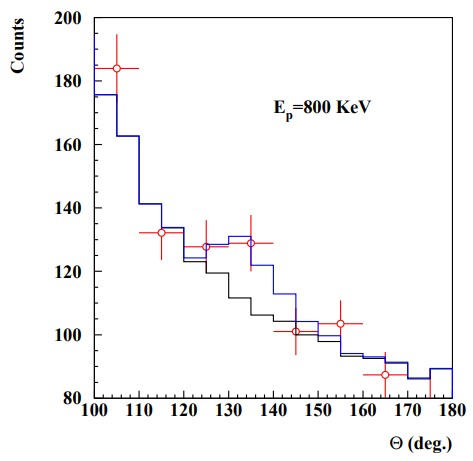
\includegraphics[width=\textwidth]{atomki_be.png}
						\caption{Experimental $e^+e^-$ pair correlations measured in the~\iso{Li}{7}$(p,e^+e^-)$\iso{Be}{8} reaction with $|y| \leq 0.5$ (closed circles) and $|y| \geq 0.5$ (open circles)~\cite{atomki_be}.}
						\label{fig:atomki_be}
					\end{subfigure}
					\hfill
					\begin{subfigure}[t]{0.42\textwidth}
						\centering
						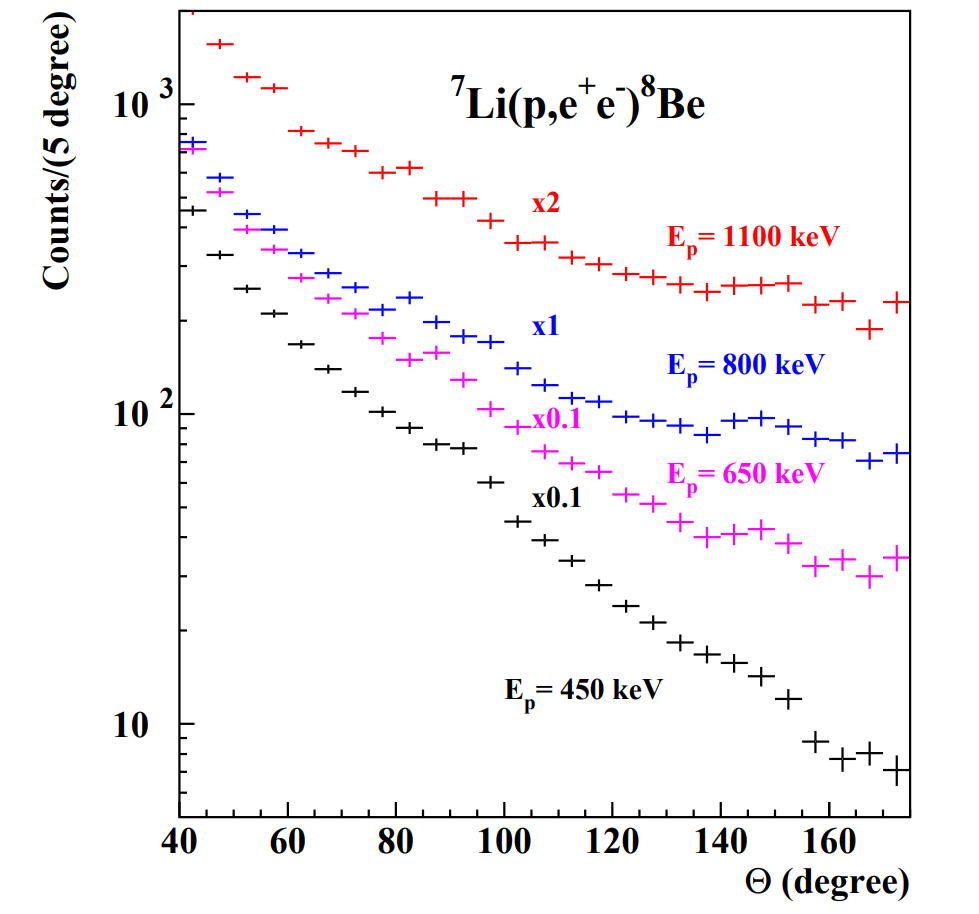
\includegraphics[width=\textwidth]{atomki_be2.png}
						\caption{Experimental $e^+e^-$ pair correlations measured in the~\iso{Li}{7}$(p,e^+e^-)$\iso{Be}{8} reaction with the~improved setup for different proton beam energies~\cite{atomki_be2}.}
						\label{fig:atomki_be2}
					\end{subfigure}
					\begin{subfigure}[t]{0.45\textwidth}
						\centering
						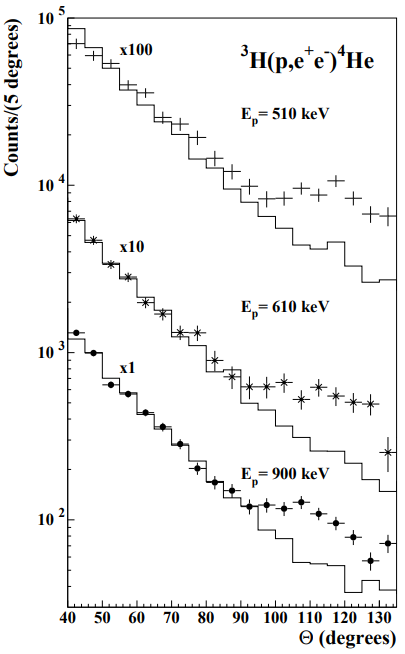
\includegraphics[width=\textwidth]{atomki_he.png}
						\caption{Experimental $e^+e^-$ pair correlations measured in the~\iso{H}{3}$(p,e^+e^-)$\iso{He}{4} reaction with $|y| \leq 0.3$ for different proton beam energies~\cite{atomki_he2}.}
						\label{fig:atomki_he}
					\end{subfigure}
					\hfill
					\begin{subfigure}[t]{0.45\textwidth}
						\centering
						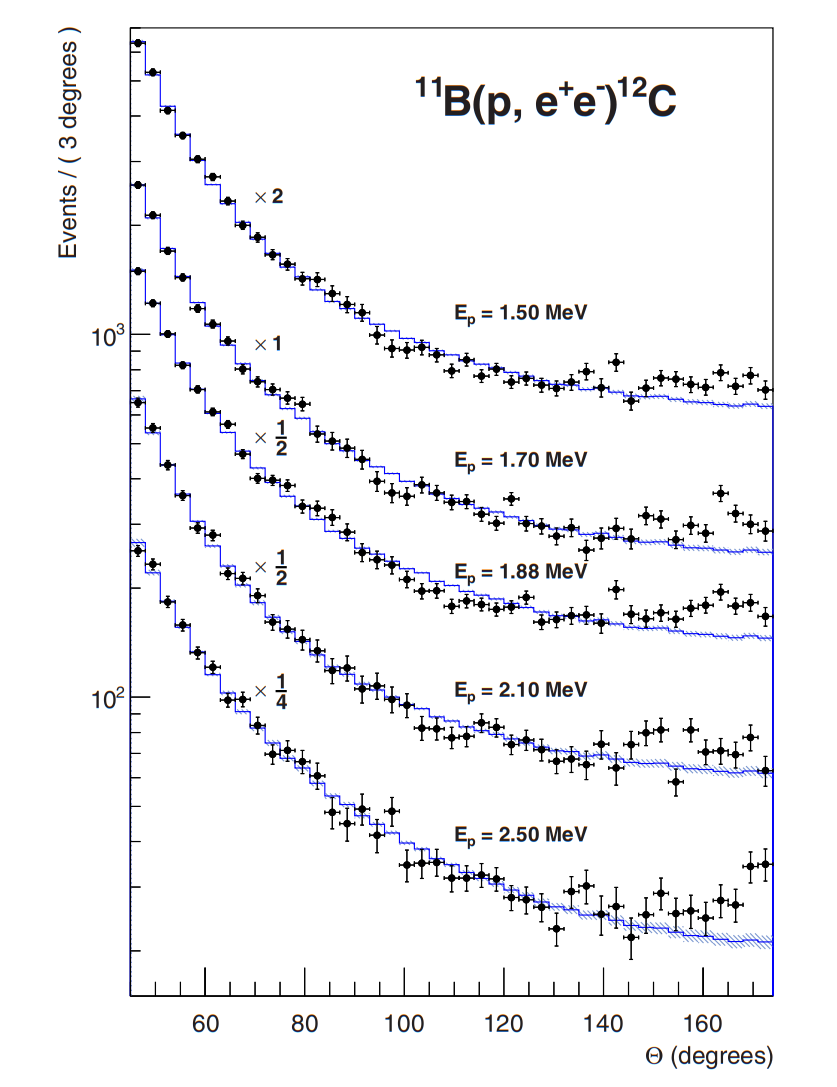
\includegraphics[width=\textwidth]{atomki_c.png}
						\caption{Experimental $e^+e^-$ pair correlations measured in the~\iso{B}{11}$(p,e^+e^-)$\iso{C}{12} reaction for different proton beam energies~\cite{atomki_c}.}
						\label{fig:atomki_c}
					\end{subfigure}
					\caption{The~ATOMKI anomalous \ac{IPC} measured for different nuclei.}
					\label{fig:atomki}
				\end{figure}
			
			Possible explanations of the~anomaly include experimental effects, higher order processes in the Standard Model~\cite{kalman,aleksejevs} or even a~protophobic fifth force mediated by a~new 17~MeV boson X17~\cite{feng}.
		
		\subsection{Other Experiments}
			Since the ATOMKI measurements, several experiments have been initiated to attempt to replicate the results and search for the hypothetical X17 particle.
			
			\subsubsection{Two-arm $e^+e^-$ spectrometer in Hanoi}
				The anomaly in \iso{Be}{8} has been observed with $>4\sigma$ confidence by a team at the Hanoi University of Sciences for $E_p = 1225$~keV~\cite{hanoi}. They built a two\nobreakdash-arm spectrometer in collaboration with ATOMKI and calibrated it using the 17.6~MeV M1 transition. The results are shown in Figure~\ref{fig:hanoi}.
				
				\begin{figure}[h]
					\centering
					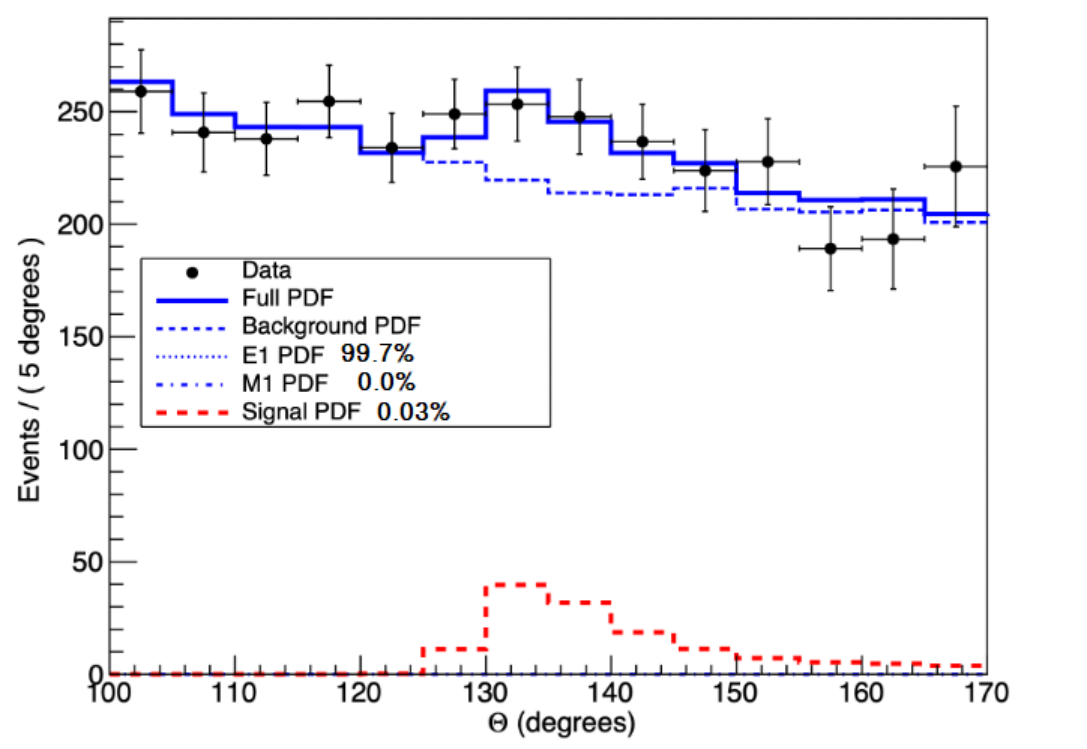
\includegraphics[width=0.75\textwidth]{hanoi.png}
					\caption{Results from the Hanoi spectrometer -- angular $e^+e^-$ pair correlations measured in the~\iso{Li}{7}$(p,e^+e^-)$\iso{Be}{8} reaction at $E_p = 1225$~keV~\cite{hanoi}.}
					\label{fig:hanoi}
				\end{figure}
			
			\subsubsection{Collisions at Nuclotron in Dubna}
				At the Joint Institute for Nuclear Research in Dubna, signal in the form of enhanced structures in the $\gamma\gamma$ spectra at $\sim 17$ and $\sim 38$~MeV invariant masses for $p+\mathrm{C}$, $d+\mathrm{C}$ and $d+\mathrm{Cu}$ reactions at momenta 5.5, 2.75, and 3.83~GeV per nucleon~\cite{dubna}. Monte Carlo simulations support the conclusion that the signals are a~consequence of a~decay of unknown particles X17 and E38.
				
			\subsubsection{The MEG II (Muon Electron Gamma) experiment}
				Experiments using the~\iso{Li}{7}$(p,e^+e^-)$\iso{Be}{8} reaction were carried out at the~Paul Scherrer Institute with the MEG II superconducting solenoid spectrometer~\cite{megii}. Analysis of the data with $E_p = 1080$~keV exciting both of the resonances (beam fully stopping in the target) found no significant evidence supporting the~X17 hypothesis. An upper bound (at 90\% confidence) on the X17\nobreakdash-to\nobreakdash-$\gamma$ branching ratio was set at $1.2\cdot10^{-5}$ for the 18.15~MeV state (larger than the ratio $5.8\cdot10^{-6}$ obtained by ATOMKI in 2016).
			
	
	\section{X17 Project at IEAP CTU}
	\label{sec:IEAP}
		\textcolor{red}{Short summary of our goals, maybe mention the~grant.}
		\textcolor{red}{\begin{itemize}
				\item \iso{Li}{7} or \iso{T}{3} target, proton beam energies to be used to excite above mentioned states, energy range (detector should be able $> 4$ MeV)
				\item three layers (TPX3, MWPC, TPC)
				\item multiple scattering problem (TPX3 in vacuum tube, carbon tube with thinned aluminum or Kapton windows, MWPC for exit point + triggering/coincidence)
				\item TPC -- energy, particle recognition (energy loss per unit distance), \textbf{more details in the next chapter}
				\item CAD drawing (with coordinate system defined in the next chapter, more figures will be there probably)
				\item TPX3 details: short description, maybe a mention of the tests
				\item couple of MWPC details could be above, TPC details in the next chapter
		\end{itemize}}